\documentclass{article}
\usepackage{amsmath}
\usepackage{graphicx}
\usepackage{listings}
\newcommand{\includecode}[2][c]{\lstinputlisting[caption=#2, escapechar=, language=#1]{#2}}
\usepackage{minted}

\begin{document}
\lstset{language=C} 
\title{Introducing Dynamic Walls in an Integer Lattice Gas Simulation}
\author{David Jedynak}
\maketitle

\begin{abstract}
The purpose of this project is to integrate dynamic shapes into an Integer Lattice Gas Simulation. This paper will cover several  approaches to create dynamic shapes in an Integer Lattice Gas Simulation, the methods used to achieve them, and how well each approach worked. Future development ideas are also discussed.   
\end{abstract}

\section{Problem Description}
The lattice gas code simulation is currently unable to model systems with dynamic rigid objects. Having the feature to add movable walls would allow for simulation of interactions between solid physical objects and gasses. The project will begin with simple moving walls that will influence particle dynamics, but the particles will not influence the walls dynamics. Afterwards, implementing wall momentum dependent on particle collisions will be developed so the particles will be able to move the walls. The first and second approach are similar in how they are tested but they have a different random distribution for how to move particles to simulate a moving wall pushing on them. The third approach observes how the gas changes when a force pushes it though a tube. The mean particle velocity is compared to a theoretical value.
\section{Background}

In order to have complex dynamic shapes, simple dynamic walls need to be achieved. A good place to start is with a static wall. There already exists a method of creating static walls in an Integer Lattice Gas Simulation by selectively inverting particle velocities based on their position in the Lattice grid. Each lattice site has 9 different velocity states particles can exist in.

\begin{table}[]
\centering
\caption{Different velocity states in each Lattice Cell, the maximum velocity amplitude in any one direction is 1}. x and y are the Cartesian coordinates of the Lattice in the Grid. 
\label{my-label}
\begin{tabular}{lllll}
	$n[x][y][0] = (-v_x,+v_y)$ & $n[x][y][1] = (0,+v_y)$ & $n[x][y][2] = (+v_x,+v_y)$ \\
	$n[x][y][3] = (-v_x,0)$ & $n[x][y][4] = (0,0)$ & $n[x][y][5] = (+v_x,0)$ \\
	$n[x][y][6] = (-v_x,-v_y)$ & $n[x][y][7] = (0,-v_y)$ & $n[x][y][8] = (+v_x,-v_y)$ \\ 
\end{tabular}
\end{table}

Particles can be reflected by swapping the number of particles in two of these velocity states. Horizontal walls are produced by switching indexes [0,1,2] with [8,7,6] respectively. Vertical walls are produced by switching [0,3,6] with [8,5,2] respectively.

\vspace{5mm}
Here is some code defining the links to produce a horizontal wall. A vertical wall can be produced by changing the values being assigned to links[linkcount][0:2] = [0 3 6] and the dimension being iterated over in the for loop:\newline
\begin{minted}{c}
//horizontal walls
  for (int x=x0; x<x1+1; x++){
    	links[linkcount][0] = x; //x-position
    	links[linkcount][1] = yy2;
    	links[linkcount][2] = 0;
    	linkcount++;
    	links[linkcount][0] = x; //x-position
    	links[linkcount][1] = yy2;
    	links[linkcount][2] = 1;
    	linkcount++;
    	links[linkcount][0] = x; //x-position 
    	links[linkcount][1] = yy2;
    	links[linkcount][2] = 2;
    	linkcount++;
  }
\end{minted}
\vspace{5mm}
Here is the code that switches the number of particles between lattice velocity states for the static walls. Note that the momentum imparted on the wall can be calculated.\newline
\begin{minted}{c}
void bounceback(){
  dynamic_wall_momentum_x = 0;
  dynamic_wall_momentum_y = 0;
  static_wall_momentum_x = 0;
  static_wall_momentum_y = 0;
  
  for (int lc=0; lc<linkcount; lc++){
    //quantity of partices
    int x=links[lc][0];
    int y=links[lc][1];
    //velocity
    int v=links[lc][2];
    int vx=v%3-1;
    int vy=1-v/3;
    int tmp= n[x+vx][y+vy][v];
    //summing all momemtums
    static_wall_momentum_x += -2*vx*(n[x][y][8-v]-tmp);
    static_wall_momentum_y += -2*vy*(n[x][y][8-v]-tmp);
    //swapping the particles trying to enter and leave to have the effect of a wall
    n[x+vx][y+vy][v]= n[x][y][8-v];
    n[x][y][8-v]=tmp;		
	}
}
\end{minted}
\vspace{5mm}



\begin{figure}[H]
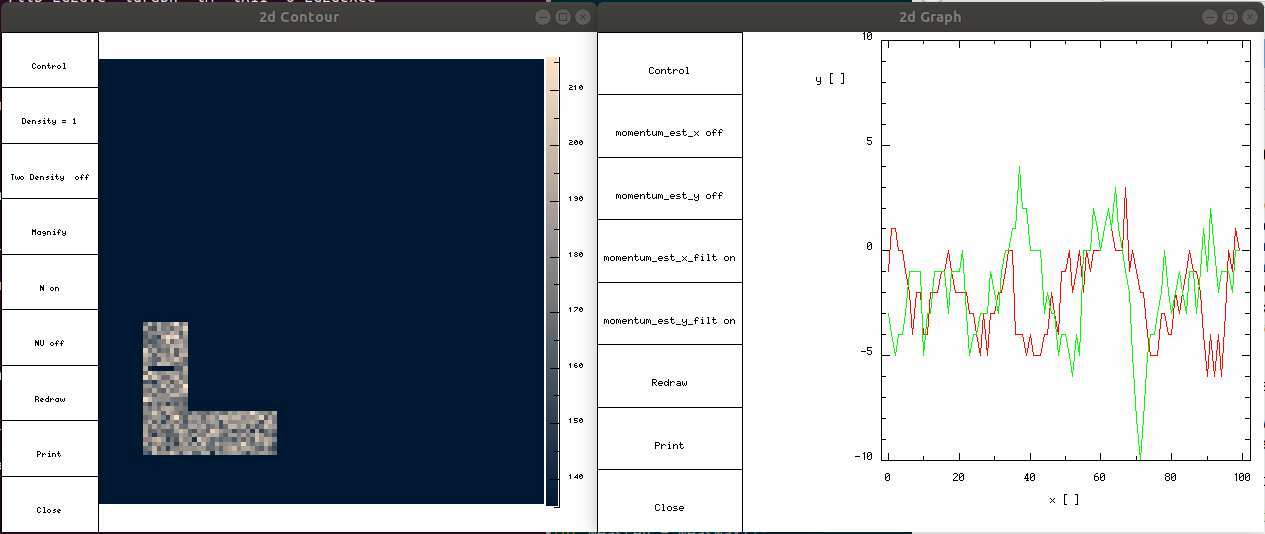
\includegraphics[scale=0.2]{p1_noleakage.png}
\caption{\label{fig} Here are several horizontal and vertical walls produced using the approach described above. The walls are containing the particles from leaving the shape. On the right hand side, there are graphs for the x and y momentum being imparted on the walls}
\end{figure}

\section{Methods}

\subsection{Approach 1}

The first approach taken to creating a moving wall was to move a wall very slowly with its velocity being much less than 1. The wall will move either dependently based on the momentum imparted on the wall due to particle collisions, or a set velocity will be given to wall.
 $$\frac{\sum_{n=1}^{nmax} -2*\textrm{net particles reflected}}{\textrm{wall mass}} = \textrm{wall velocity}$$
\vspace{5mm}

Code for calculating the wall momentum and resulting velocity
\begin{minted}{c}
    //summing all momemtums
    dynamic_wall_momentum_x += -2*vx*(n[x][y][8-v]-tmp);
    dynamic_wall_momentum_y += -2*vy*(n[x][y][8-v]-tmp);

	if(dynamic_wall_control_on == 0){
    		dynamic_wall_vx = dynamic_wall_momentum_x/wall_mass;
    		dynamic_wall_vy = dynamic_wall_momentum_y/wall_mass;
	}
\end{minted}
\vspace{5mm}

As the wall moves, it would "pass over" particles due to rest particles in the $n[x][y][0]$ state. To compensate for this, a random number of particles would be added to either side of the wall depending on the wall's velocity and the density of the particles surrounding the wall. For simplicity, a flat distribution was used ranging from 0 to the smaller density of particles on either side of the wall. This is necessary to prevent negative densities. This number of particles is refereed to as "flow".

$$
\textrm{Expected value of flow}$$\\
$$<flow> = \textrm{particle density * wall velocity}$$\\
$$0 < flow < \textrm{min particle density}$$\\




The code for calculating flow is defined below. First the 2 particle densities are assigned to 2 temp variables. The smaller of the two is used as the max value in the random distribution. 
\begin{minted}{c}
  int tmp_0 = n[(((vx+x)%XDIM)+XDIM)%XDIM][((y+vy)%YDIM+YDIM)%YDIM][8-v];
    int tmp = n[(((vx+x)%XDIM)+XDIM)%XDIM][((y+vy)%YDIM+YDIM)%YDIM][v];
	int max_random = 1;
	if(tmp > tmp_0){
		max_random = tmp_0;
		}
	else{
		max_random = tmp;
		}
	if(max_random > 0){
		flow = (rand()%max_random)*dynamic_wall_vx;
		}
	else{
		flow = 0;
		}
\end{minted}
\vspace{5mm}
The following wall momentum is then:
\begin{minted}{c}
    dynamic_wall_momentum_x += -2*vx*(n[x][y][8-v]-tmp+flow);
    dynamic_wall_momentum_y += -2*vy*(n[x][y][8-v]-tmp);
    \end{minted}
\vspace{5mm}


\vspace{5mm}
Adding the flow to the lattice sites to produce a moving wall
\begin{minted}{c}
    //swapping the particles trying to enter and leave to have the effect of a wall
    n[(((vx+x)%XDIM)+XDIM)%XDIM][((y+vy)%YDIM+YDIM)%YDIM][v] = n[(((x)%XDIM)+XDIM)%XDIM][((y)%YDIM+YDIM)%YDIM][8-v] - flow;
    n[(((x)%XDIM)+XDIM)%XDIM][((y)%YDIM+YDIM)%YDIM][8-v] = tmp + flow;		
    \end{minted}
\vspace{5mm}

\subsection{Results}

Initial results were promising, but this approach did not factor in the number of particles at rest position, so there was significant particle leakage.

\begin{figure}[H]
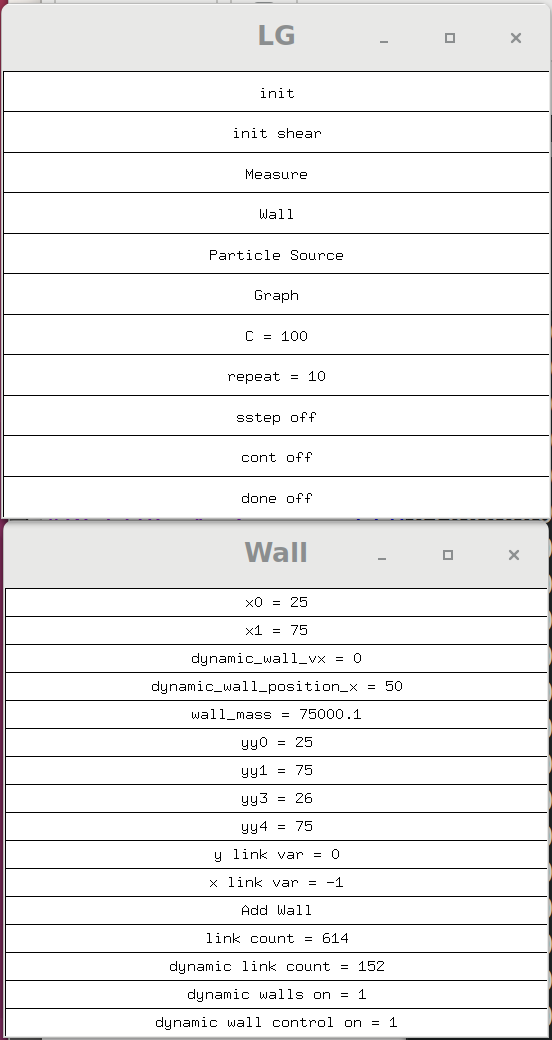
\includegraphics[scale=0.35]{A1_p0.png}
\caption{\label{fig} Settings for the simulation}
\end{figure}

\begin{figure}[H]
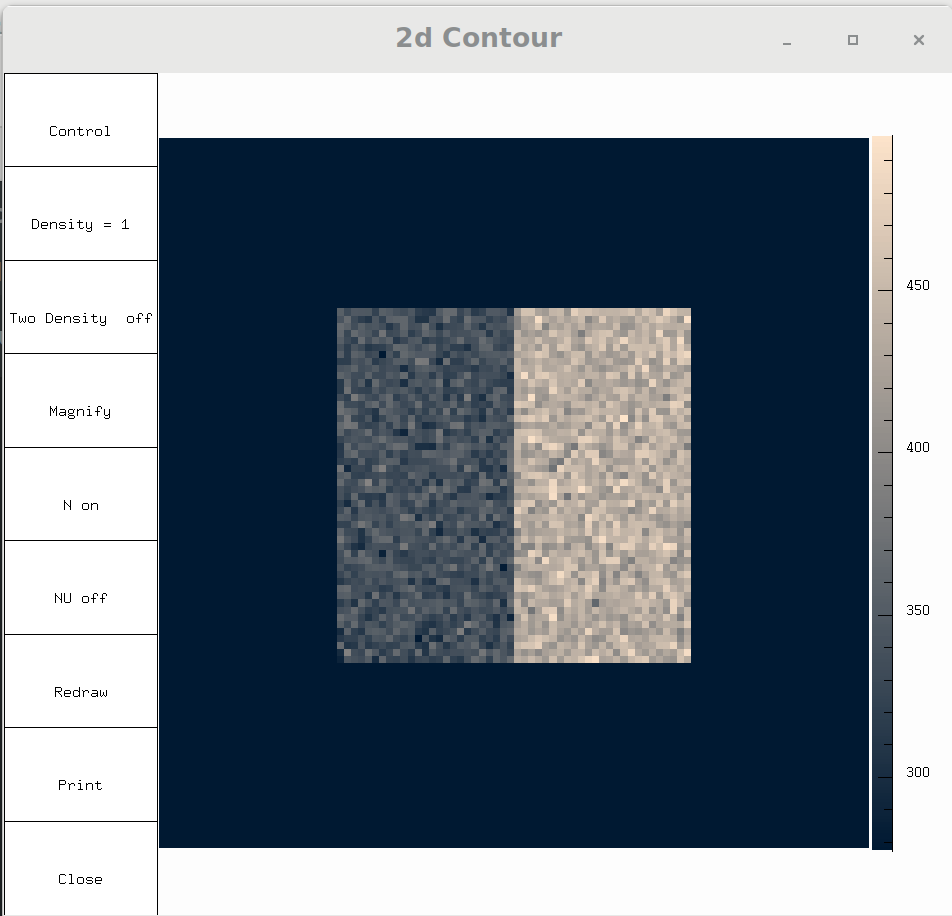
\includegraphics[scale=0.35]{A1p1.png}
\caption{\label{fig}  A box produced with static walls with one vertical dynamic wall in the center. The density on the right is 15*9 and the density on the right is 10*9. The wall is being held at position 50}
\end{figure}

\begin{figure}[H]
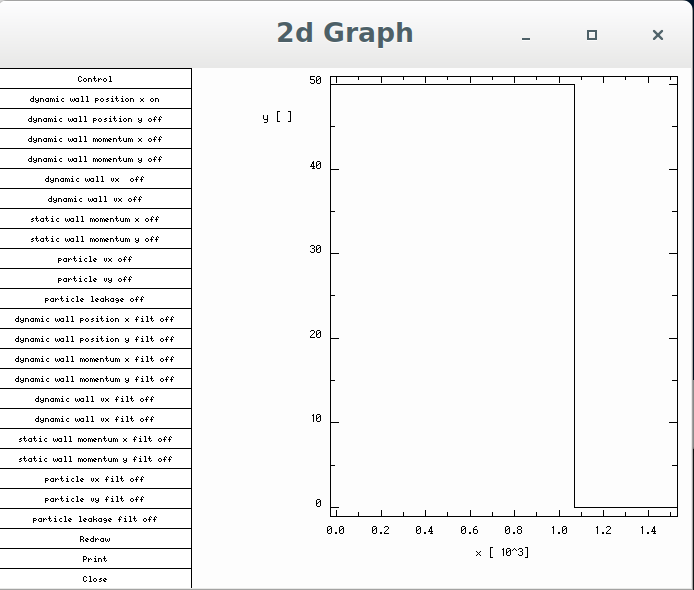
\includegraphics[scale=0.35]{A1p2.png}
\caption{\label{fig} Graph of the dynamic wall x position}
\end{figure}

\begin{figure}[H]
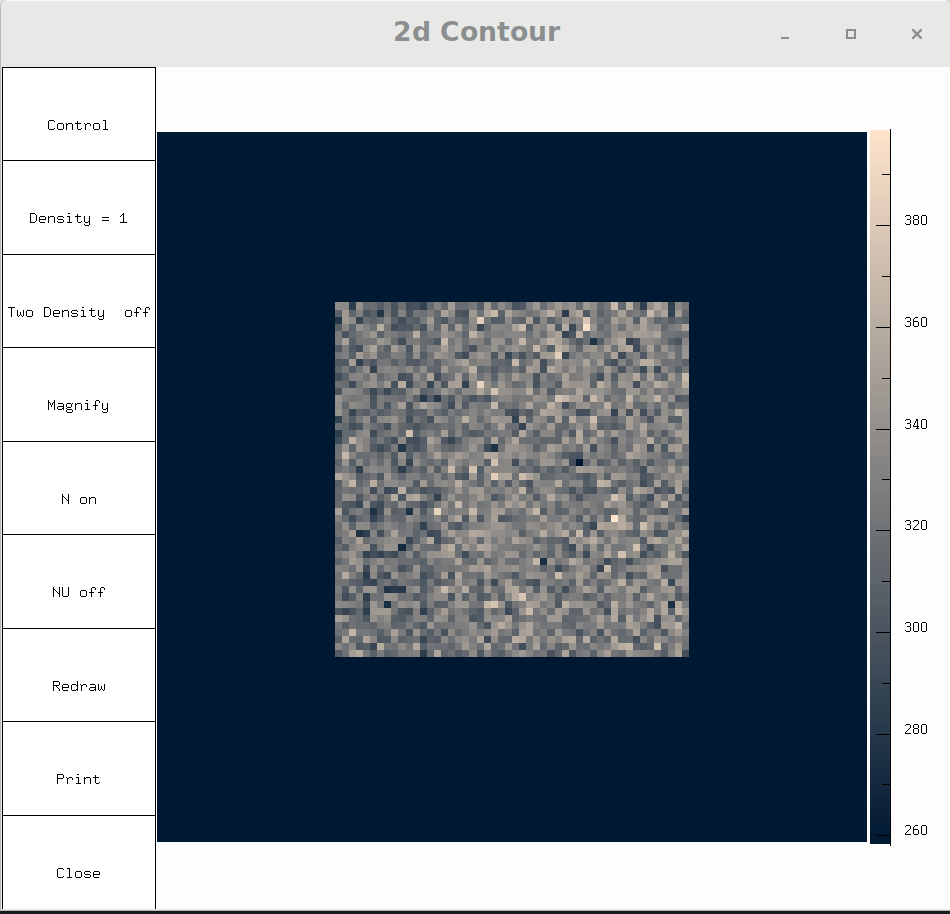
\includegraphics[scale=0.35]{A1p3.png}
\caption{\label{fig} The force keeping the dynamic wall is removed and the wall moved towards equilibrium, but it passes the theoretical equilibrium point: 45. This error is due to leakage from rest particles}
\end{figure}

\begin{figure}[H]
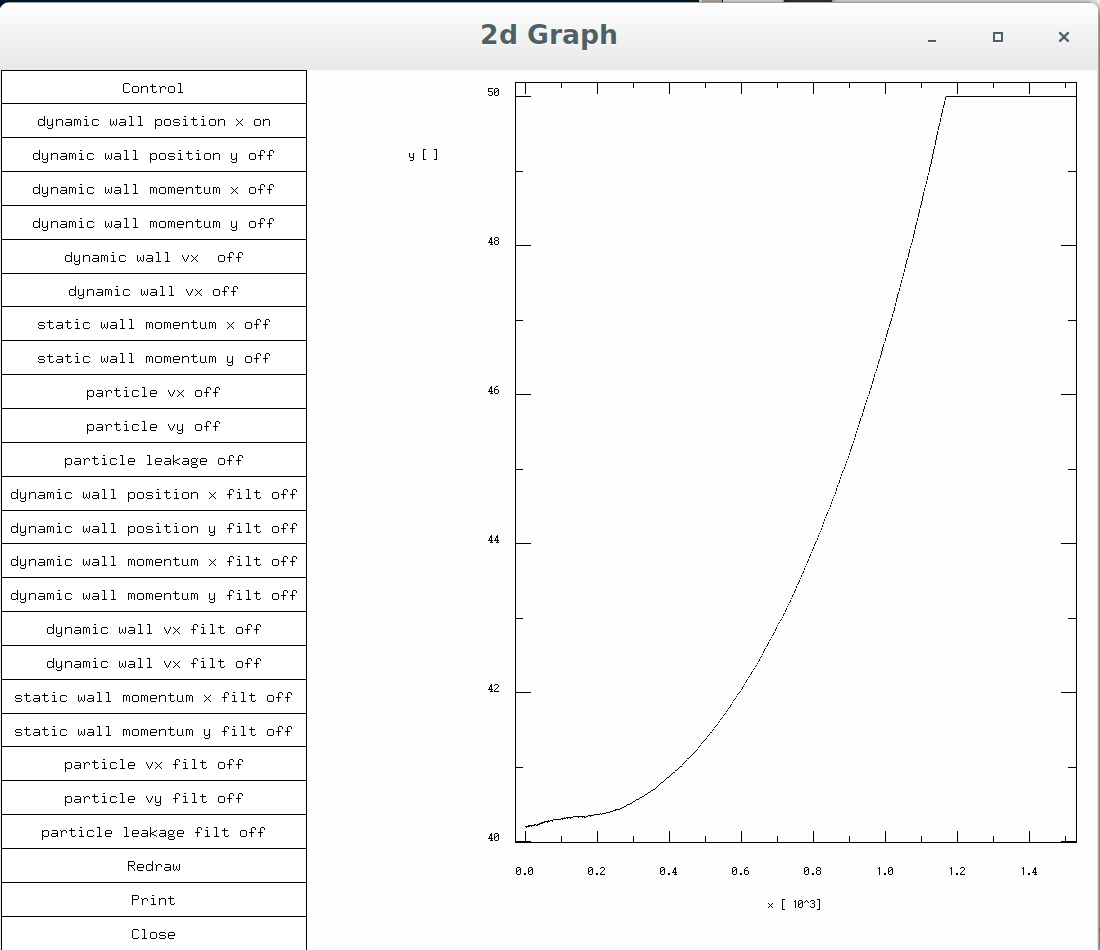
\includegraphics[scale=0.35]{A1p4.png}
\caption{\label{fig} Graph of the walls x position as it moved towards equilibrium overt time}
\end{figure}

\begin{figure}[H]
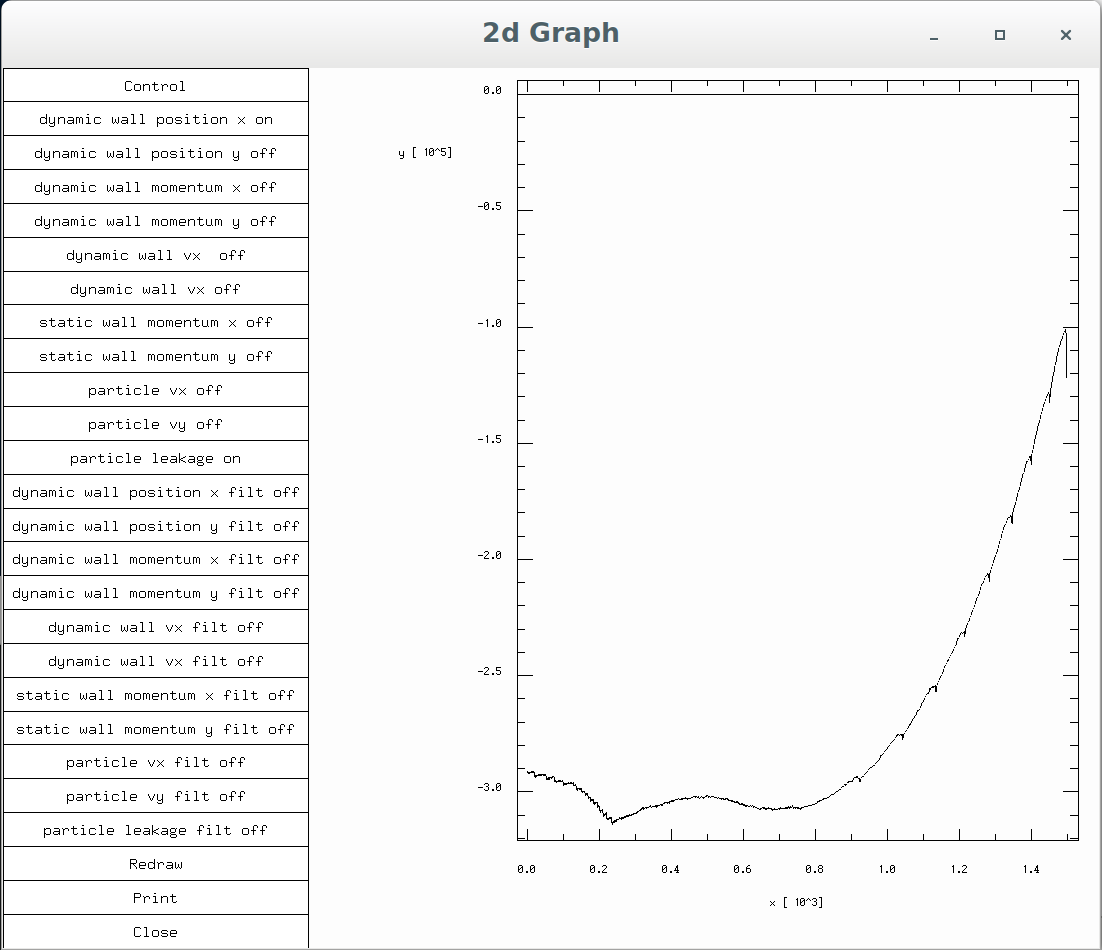
\includegraphics[scale=0.35]{A1p5.png}
\caption{\label{fig} The particles leaking through the dynamic wall as the wall moved. Note how the leakage is proportional to the walls velocity.}
\end{figure}

\subsection{Approach 2}
Approach 2 is very similar to the first approach, but the primary focus was to ensure that all the particles would be removed from the lattice site by the time the wall would exit to the next lattice site. The wall has a real number for its position whereas the lattice grid is integer, so the wall will be transitioning between lattice sites. In more detail, the probability that $ pr * \textrm{particle density}$ number of particles will be moved is defined by $$pr = \frac{\textrm{Wall Vx}}{1-(\textrm{real(Wall x) - int(Wall x)})}$$. As the wall becomes closer and closer to changing lattice sites, the probability that all the particles will be moved to the next lattice site will converge to one. This is only for a case where a wall is moving to the right. This can be reproduced for a left moving wall, but was not in this program for simplicity.

\vspace{5mm}
Code added for determining the flow of particles as the wall moves.
\begin{minted}{c}
int tmp = n[x_v_b][y_v_b][v];
int iwp = dynamic_wall_position_x;//integer wall position
int flow = 0;//particles to be moved
		
double pr = dynamic_wall_vx/(1-(dynamic_wall_position_x - iwp));
//probability that p*pr particles will be moved
		if(rand()%1000 <= 1000*pr){
			flow = pr*n[x_b][y_b][v];
			n[x_b+1][y_b][v] +=flow;
			n[x_b][y_b][v] -=flow;
		}
 \end{minted}
\vspace{5mm}

\subsection{Results}

This approach had a similar amount of leaking particles as the first approach. 

\begin{figure}[H]
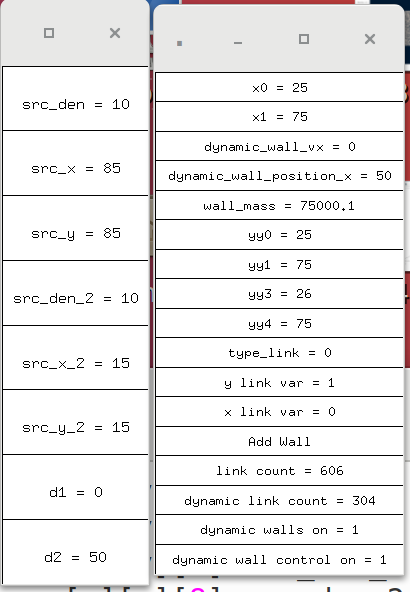
\includegraphics[scale=0.35]{A11p0.png}
\caption{\label{fig} Settings for the simulation}
\end{figure}


\begin{figure}[H]
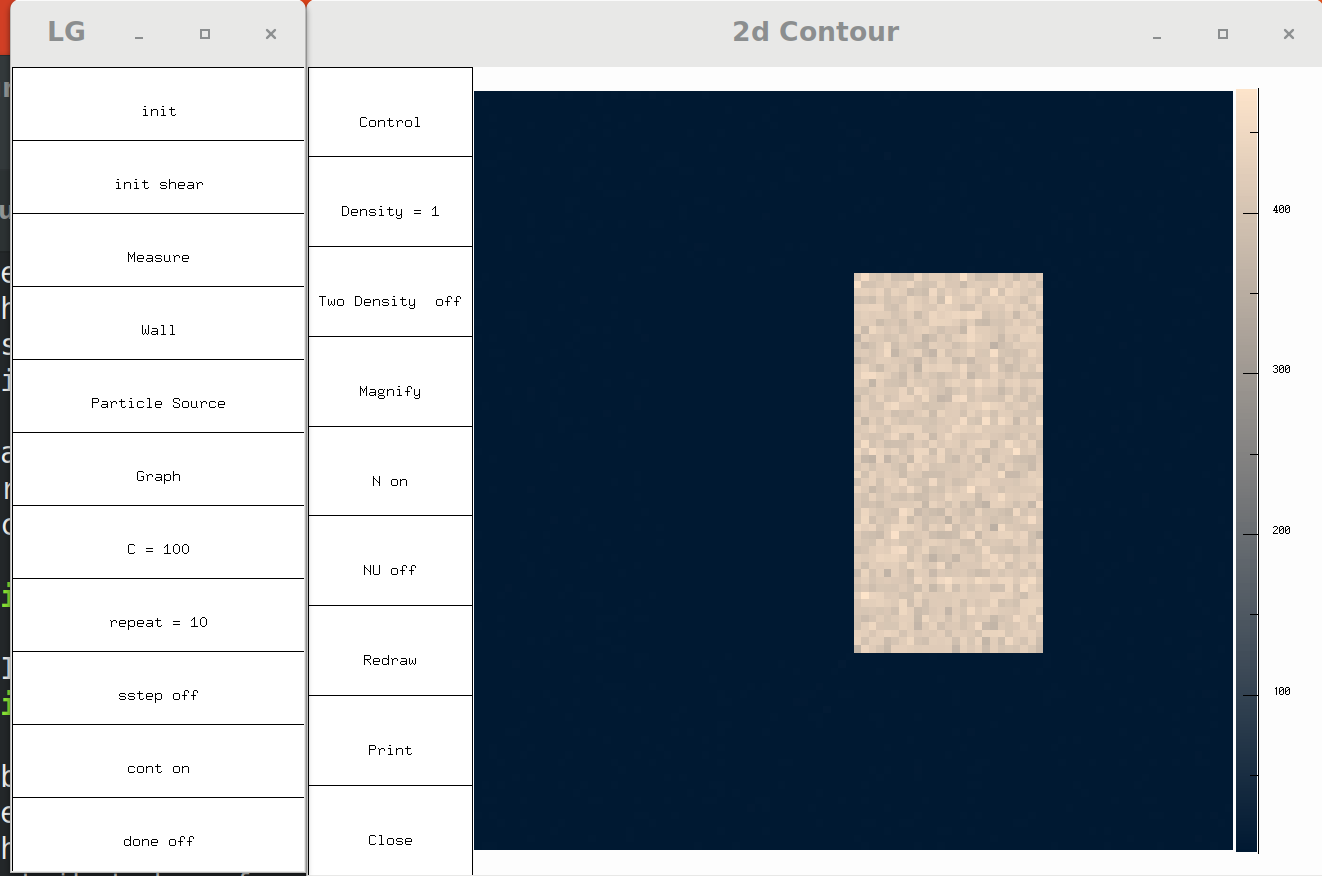
\includegraphics[scale=0.35]{A11p2.png}
\caption{\label{fig} A box produced with static walls with one vertical dynamic wall in the center. The density on the right is 50*9 and the density on the right is 0. The wall is being held at position 50. This experiment is being done to test if the wall will leak any particles. }
\end{figure}


\begin{figure}[H]
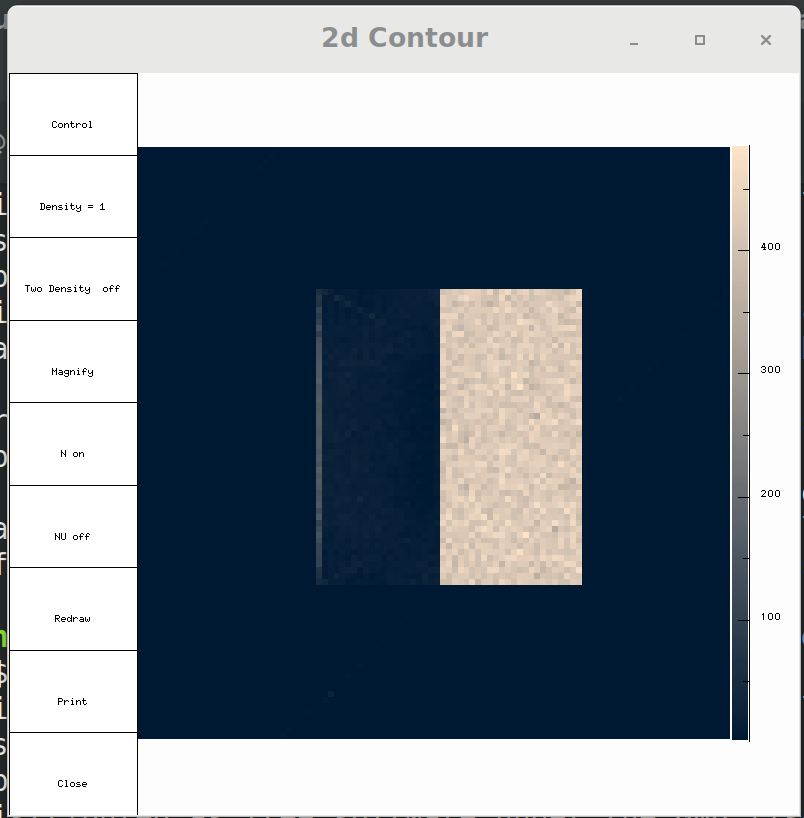
\includegraphics[scale=0.35]{A11p5.png}
\caption{\label{fig} The wall begins to move with velocity of 0.02 in the positive x direction. Notice how a notable wave of particles are being leaked when the wall changes lattice sites.}
\end{figure}

\begin{figure}[H]
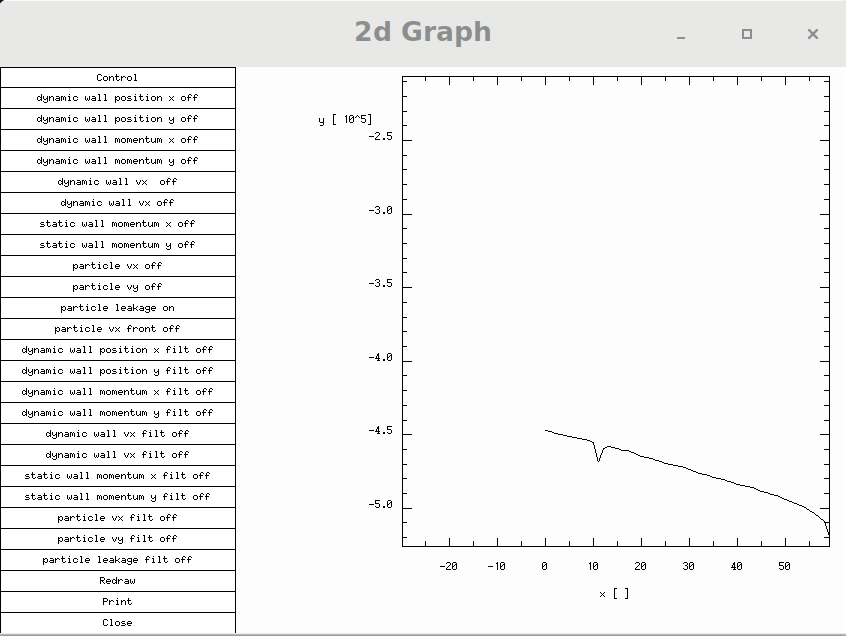
\includegraphics[scale=0.35]{A11p3.png}
\caption{\label{fig} Graph of the particles being leaked by the wall over time}
\end{figure}

\begin{figure}[H]
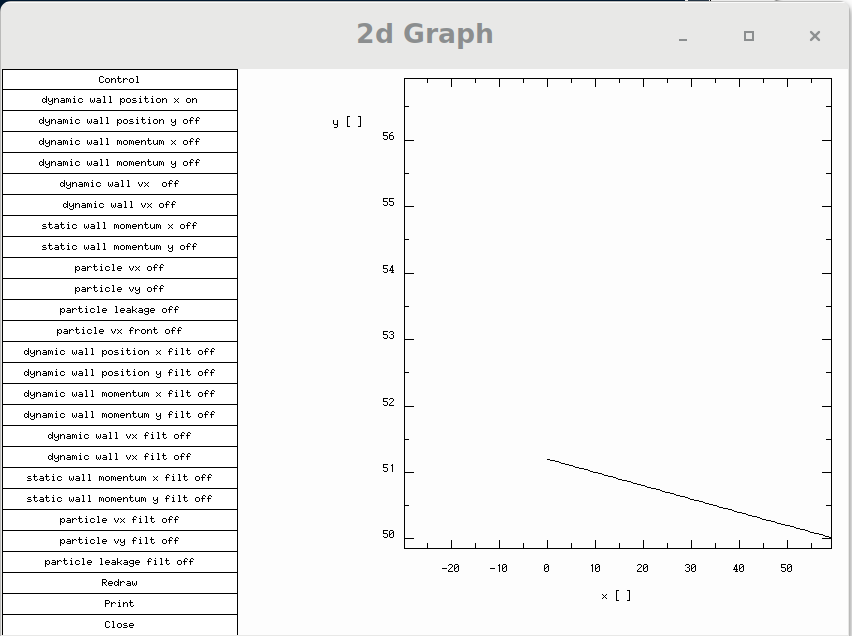
\includegraphics[scale=0.35]{A11p4.png}
\caption{\label{fig} Graph of the walls x position as it moved towards equilibrium overt time}
\end{figure}

\subsection{Approach 3}

This approach tried to simplify the program by restricting the motions of the wall, then in this specific case, the walls dynamics can be tested and verified if possible. Rest particles are still known to be causing issues, so to remove them, the walls will move into a region where there are no particles. This simulation will apply a force to particles confined by 2 walls with periodic boundary conditions allowing particles to flow from one end of the tube to the other. The walls will be static to begin with and dynamic later. The force will be applied by moving a random amount of particles from the lattice velocity states of [2 5 8] to [0 3 6]. To validate the dynamics of the simulation, the mean particle velocity with respect to the cross section of the tube will be measured in the simulation and compared to a theoretical value derived from the Navier Stokes equation for fluid dynamics.

\begin{equation}
\frac{\partial \rho}{\partial t} + \frac{\partial(\rho u_{i})}{\partial x_{i}} = \nabla(\rho) + \upsilon *\nabla(\nabla(U)+(\nabla(U)T))
\end{equation}

The partial for $\rho$ and $\rho u_{i}$ can be set to zero.
This gives us:

\begin{equation}
0 = \nabla(\rho) + \upsilon *\nabla(\nabla(U)+(\nabla(U)T))
\end{equation}

$$ \nabla(\rho) = F$$ 

\begin{equation}
0 = F + \upsilon *\nabla(\nabla(U_x))
\end{equation}

Solving the differential equation for $U_x$ (mean velocity) above gives us:

\begin{equation}
U_x =\frac{F}{2*\upsilon}*(x(x-L))
\end{equation}
\vspace{5mm}
Where L is the length of the tube in Lattice sites.\\
\vspace{5mm}
For C (Particle Collisions) the viscosity is: \\
\begin{equation} 
 \upsilon = \frac{1}{6}
 \end{equation}

This is the theoretical curve for the mean x velocity in the tube
\begin{equation}
U_x =\frac{F*6}{2}*(x(x-L)) 
\end{equation}

\vspace{5mm}
The expected value of particles being moved by a set force is related to the equation below.  
\begin{equation}
<\textrm{particles moved}> = force*\rho
\end{equation}

\vspace{5mm}
Code for applying a force to the particles. The variable "particle flip w" is the force applied.
\begin{minted}{c}
void moveParticles(){
for(int x = 0;x<xdim;x++){
	for(int y = 0;y<ydim;y++){
		int flip_parts = particle_flip_w*((double)rand()/RAND_MAX)*n[x][y][5];
		n[x][y][3] += flip_parts;
		n[x][y][5] -= flip_parts;
		flip_parts = particle_flip_w*((double)rand()/(double)RAND_MAX)*n[x][y][8];
		n[x][y][6] += flip_parts;
		n[x][y][8] -= flip_parts;
		flip_parts = particle_flip_w*((double)rand()/(double)RAND_MAX)*n[x][y][2];
		n[x][y][0] += flip_parts;
		n[x][y][2] -= flip_parts;
		}
	}
}
 \end{minted}
\vspace{5mm}

Code for calculating the theoretical curve and measuring the mean x velocity of the particles

\vspace{5mm}
\begin{minted}{c}
void measure_function(){
particle_vx = 0;
particle_vy = 0;
int total_particles = 0;
for(int i = 0; i < YDIM -1;i++){
	total_particles = 0;
	measure_particle_velocity_front[i] = 0;
	for(int x0 = 0;x0<xdim;x0++){
		measure_particle_velocity_front[i] += n[x0][i][5]+n[x0][i][2]+n[x0][i][8] -
		n[x0][i][3]-n[x0][i][0]-n[x0][i][6];			
			 for(int v = 0;v<9;v++) total_particles += n[x0][i][v];	
			}
		//find average particle velocity
		if(total_particles > 0){
			measure_particle_velocity_front[i] = 
			(double(measure_particle_velocity_front[i]/total_particles);//+shift[i];
			theoretical_particle_vx_front[i] = 	
			(double(particle_flip_w*6.0/9.)*(i-25)*(i-75);

			}
		else{
			measure_particle_velocity_front[i] = 0;
			theoretical_particle_vx_front[i] = 0;
			}
		
		measure_particle_force_front[i] = (measure_particle_velocity_front[i]
		 measure_particle_velocity_front_last[i]);	
		measure_particle_velocity_front_last[i] = measure_particle_force_front[i];
		}
	}

 \end{minted}
\vspace{5mm}


\subsection{Results}
There is a very large difference in the two mean velocity in the x directions, but the measured mean x velocity does show a parabolic profile like the theory suggests. Additionally, there were no simulations with dynamic walls because the simulation needs to work first with static walls, before moving on to dynamic walls.

\begin{figure}[H]
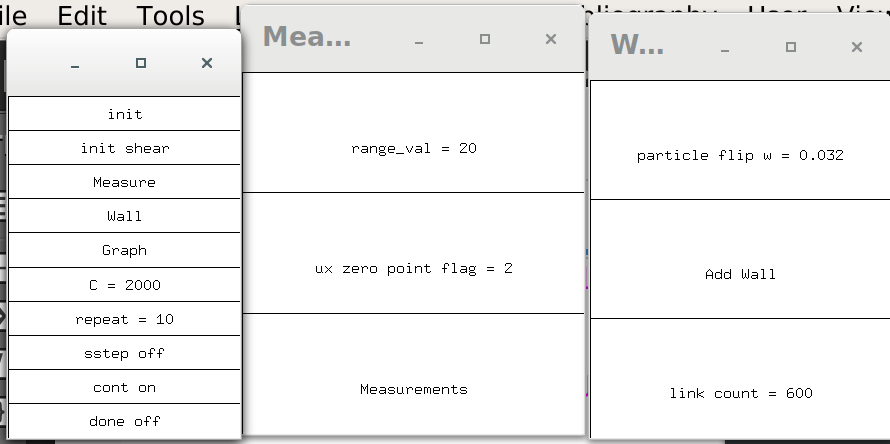
\includegraphics[scale=0.35]{A2p1.png}
\caption{\label{fig} Simulation settings}
\end{figure}

\begin{figure}[H]
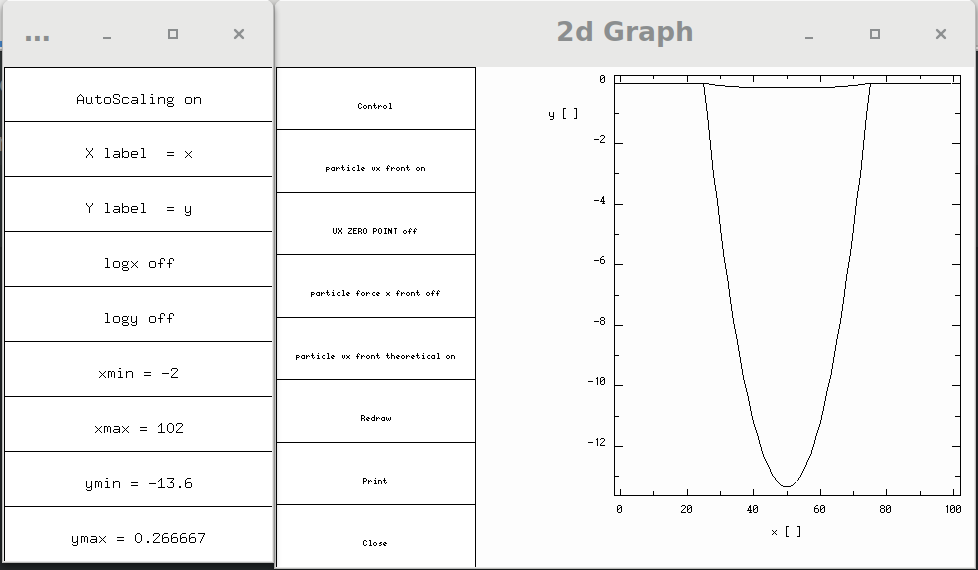
\includegraphics[scale=0.35]{A3p0.png}
\caption{\label{fig} Theoretical and measured mean particle x velocity}
\end{figure}

\begin{figure}[H]
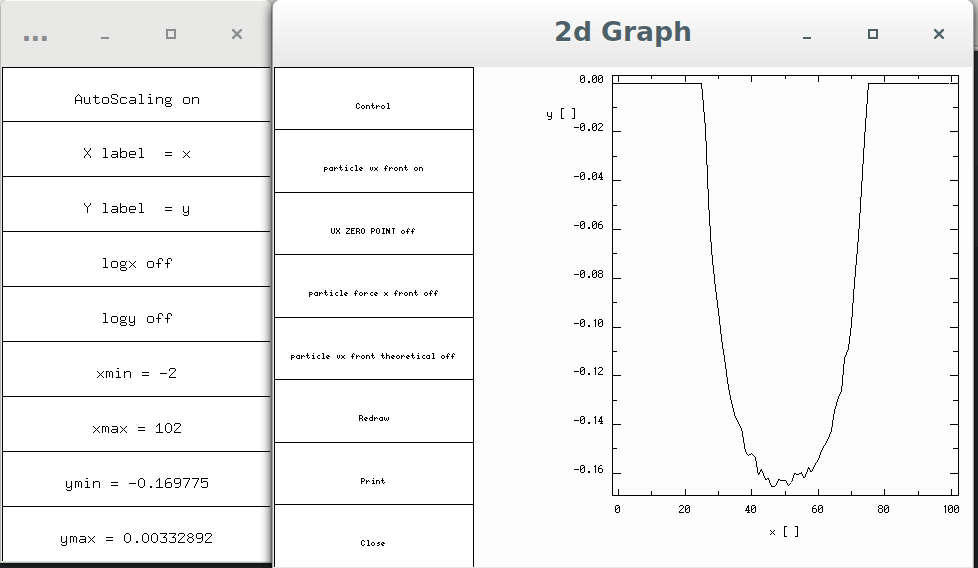
\includegraphics[scale=0.35]{A2p3.png}
\caption{\label{fig} Measured mean particle velocity x}
\end{figure}


\section{Conclusion}

Although there is significant error for approaches 1 and 2 because there are on the order of a couple hundred particles leaking per iteration in a simulation that has around total particles the walls do appear to work reasonably for short periods of time i.e. several hundred iterations. If the leaking of the particles problem was resolved, work could continue on creating complex shapes out of multiple walls and see how they interact with the simulated gas. this would work The 3rd approach was also significantly off by roughly a factor of 50, but it might work if the number of particles flipped was determined by its integer component and its probability of occurring was related to the decimal component. Future progress on this topic should try to narrow its scope to try and lower complexity so the nature of the problem of the problem can become more clear.


\appendix
\section{Code}
\subsection{Code for Approach 1}
\lstinputlisting[language=C]{/home/david/Documents/Computational_Physics/Lattice_Gas_Movable_Links/Moving_Wall/LG2d.c}
\subsection{Code for Approach 2}
\lstinputlisting[language=C]{/home/david/Documents/Computational_Physics/Lattice_Gas_Movable_Links/Moving_Wall_1/LG2d.c}
\subsection{Code for Approach 3}
\lstinputlisting[language=C]{/home/david/Documents/Computational_Physics/Lattice_Gas_Movable_Links/Moving_Wall_2/LG2d.c}
\end{document}
  

\end{document}

